\documentclass[12pt,a4paper]{article}
\usepackage[utf8]{inputenc}
\usepackage[T1]{fontenc}
\usepackage{geometry}
\usepackage{graphicx}
\usepackage{amsmath,amssymb}
\usepackage{listings}
\usepackage{xcolor}
\usepackage{hyperref}
\usepackage{booktabs}
\usepackage{float}
\usepackage{tikz}
\usepackage{algorithm}
\usepackage{algpseudocode}
\usepackage{multirow}
\usepackage{subcaption}

\geometry{margin=1in}

% Code listing style
\definecolor{codegreen}{rgb}{0,0.6,0}
\definecolor{codegray}{rgb}{0.5,0.5,0.5}
\definecolor{codepurple}{rgb}{0.58,0,0.82}
\definecolor{backcolour}{rgb}{0.95,0.95,0.92}

\lstdefinestyle{mystyle}{
    backgroundcolor=\color{backcolour},   
    commentstyle=\color{codegreen},
    keywordstyle=\color{magenta},
    numberstyle=\tiny\color{codegray},
    stringstyle=\color{codepurple},
    basicstyle=\ttfamily\footnotesize,
    breakatwhitespace=false,         
    breaklines=true,                 
    captionpos=b,                    
    keepspaces=true,                 
    numbers=left,                    
    numbersep=5pt,                  
    showspaces=false,                
    showstringspaces=false,
    showtabs=false,                  
    tabsize=2
}
\lstset{style=mystyle}

\hypersetup{
    colorlinks=true,
    linkcolor=blue,
    filecolor=magenta,      
    urlcolor=cyan,
    pdftitle={Robot Arm Teleoperation and Control Framework},
}

\title{
    \textbf{Robot Arm Teleoperation and Control Framework} \\
    \vspace{0.5cm}
    \large A Comprehensive System for Bilateral Control, WebXR Teleoperation, \\
    and Reinforcement Learning Dataset Collection
}

\author{
    Research and Development Project Report \\
    5th Semester
}

\date{December 2025}

\begin{document}

\maketitle

\begin{abstract}
This report presents a comprehensive framework for robotic manipulator teleoperation and control, encompassing three major components: \textbf{arm-bench} (a robot arm benchmarking and control toolkit), \textbf{control\_simulator} (a MATLAB-integrated control algorithm simulator with automatic parameter tuning), and \textbf{manipulator\_teleop} (a ROS2-based teleoperation system with WebXR support). The framework supports multiple robot platforms including Interbotix arms, Franka Emika Panda, Kinova Gen3, and Open Manipulator X. Key capabilities include bilateral teleoperation, forward and inverse kinematics computation, WebXR-based immersive control, RLDS dataset recording for reinforcement learning, and sophisticated control parameter optimization. The system architecture enables seamless integration between simulation and hardware environments, facilitating research in robot learning and human-robot interaction.
\end{abstract}

\tableofcontents
\newpage

%==============================================================================
\section{Introduction}
%==============================================================================

\subsection{Background and Motivation}

The field of robotic manipulation has witnessed significant advances in recent years, driven by the convergence of improved hardware, sophisticated control algorithms, and machine learning techniques. Teleoperation remains a critical capability for tasks requiring human intuition and dexterity, ranging from surgical robotics to industrial assembly and hazardous environment operations.

This project addresses the need for a unified framework that bridges multiple aspects of robotic manipulation:
\begin{itemize}
    \item \textbf{Hardware Abstraction}: Supporting diverse robot platforms with a consistent interface
    \item \textbf{Teleoperation}: Enabling intuitive remote control through various input modalities
    \item \textbf{Control System Development}: Facilitating the design and tuning of control algorithms
    \item \textbf{Data Collection}: Supporting reinforcement learning research through standardized dataset creation
\end{itemize}

\subsection{Project Objectives}

The primary objectives of this framework are:
\begin{enumerate}
    \item Develop a modular architecture supporting multiple robotic manipulators
    \item Implement bilateral teleoperation between leader and follower arms
    \item Create WebXR-based teleoperation for immersive control using mobile devices
    \item Integrate MATLAB engine for advanced control algorithm simulation
    \item Provide automatic parameter tuning capabilities for PID, LQR, and MPC controllers
    \item Enable RLDS (Reinforcement Learning Dataset) format recording for robot learning
    \item Support bimanual manipulation with coordinated dual-arm control
\end{enumerate}

\subsection{Report Organization}

This report is organized as follows: Section 2 details the technical stack and technologies employed. Section 3 explores application domains. Section 4 presents the implementation details of each component. Section 5 demonstrates results and provides usage examples. Section 6 discusses the reinforcement learning-based bimanual control capabilities. Section 7 concludes with future directions.

%==============================================================================
\section{Technical Stack}
%==============================================================================

\subsection{Software Technologies}

The framework leverages a diverse set of technologies across multiple domains:

\subsubsection{Core Programming Languages}
\begin{itemize}
    \item \textbf{Python 3.10+}: Primary implementation language for all components
    \item \textbf{MATLAB}: Control algorithm implementation and simulation engine
    \item \textbf{JavaScript}: WebXR frontend for immersive teleoperation
\end{itemize}

\subsubsection{Robotics Middleware}
\begin{itemize}
    \item \textbf{ROS2 (Robot Operating System 2)}: Message passing, node management, and robot control
    \item \textbf{Dynamixel SDK}: Low-level motor control using Protocol 2.0
    \item \textbf{Interbotix ROS Packages}: Support for Interbotix arm series
\end{itemize}

\subsubsection{Simulation Frameworks}
\begin{itemize}
    \item \textbf{MuJoCo}: Physics simulation engine for accurate robot dynamics
    \item \textbf{Mink}: Inverse kinematics library built on MuJoCo
    \item \textbf{RViz}: 3D visualization for ROS2
\end{itemize}

\subsubsection{Web Technologies}
\begin{itemize}
    \item \textbf{FastAPI}: Asynchronous web server for WebXR backend
    \item \textbf{WebSocket}: Real-time bidirectional communication
    \item \textbf{WebXR API}: Augmented/Virtual reality support in browsers
    \item \textbf{Uvicorn}: ASGI server for FastAPI applications
\end{itemize}

\subsubsection{Scientific Computing}
\begin{itemize}
    \item \textbf{NumPy}: Numerical computing and linear algebra
    \item \textbf{SciPy}: Optimization algorithms (Differential Evolution, Nelder-Mead, Powell)
    \item \textbf{MATLAB Engine for Python}: Python-MATLAB integration
\end{itemize}

\subsection{Hardware Support}

\subsubsection{Supported Robot Arms}
\begin{table}[H]
\centering
\caption{Supported Robotic Manipulators}
\begin{tabular}{@{}llll@{}}
\toprule
\textbf{Robot} & \textbf{DOF} & \textbf{Type} & \textbf{Workspace Size} \\
\midrule
ReactorX-150 (RX150) & 5 & Interbotix & Small \\
ReactorX-200 (RX200) & 5 & Interbotix & Medium \\
ViperX-300s (VX300s) & 6 & Interbotix & Large \\
Franka Emika Panda & 7 & Industrial & Large \\
Kinova Gen3 & 6/7 & Collaborative & Large \\
Open Manipulator X (OMX) & 4/5 & ROBOTIS & Small \\
\bottomrule
\end{tabular}
\end{table}

\subsubsection{Dynamixel Motor Support}
The framework supports Dynamixel servo motors using Protocol 2.0, with comprehensive control table access for:
\begin{itemize}
    \item Position, velocity, and current control modes
    \item Real-time feedback: position, velocity, current, temperature
    \item PID gain tuning at motor level
    \item Profile velocity and acceleration settings
\end{itemize}

\subsection{System Architecture}

\begin{figure}[H]
\centering
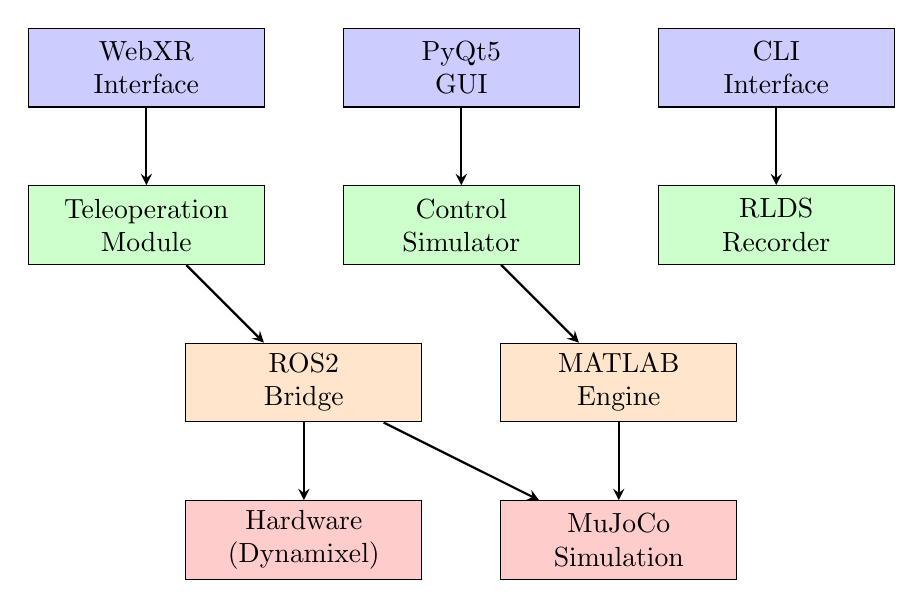
\begin{tikzpicture}[
    box/.style={rectangle, draw, minimum width=3cm, minimum height=1cm, align=center},
    arrow/.style={->, >=stealth, thick}
]
    % Top layer - User Interfaces
    \node[box, fill=blue!20] (webxr) at (0,4) {WebXR\\Interface};
    \node[box, fill=blue!20] (gui) at (4,4) {PyQt5\\GUI};
    \node[box, fill=blue!20] (cli) at (8,4) {CLI\\Interface};
    
    % Middle layer - Core Modules
    \node[box, fill=green!20] (teleop) at (0,2) {Teleoperation\\Module};
    \node[box, fill=green!20] (control) at (4,2) {Control\\Simulator};
    \node[box, fill=green!20] (record) at (8,2) {RLDS\\Recorder};
    
    % Lower layer - Hardware/Simulation
    \node[box, fill=orange!20] (ros2) at (2,0) {ROS2\\Bridge};
    \node[box, fill=orange!20] (matlab) at (6,0) {MATLAB\\Engine};
    
    % Bottom layer - Hardware
    \node[box, fill=red!20] (hw) at (2,-2) {Hardware\\(Dynamixel)};
    \node[box, fill=red!20] (sim) at (6,-2) {MuJoCo\\Simulation};
    
    % Arrows
    \draw[arrow] (webxr) -- (teleop);
    \draw[arrow] (gui) -- (control);
    \draw[arrow] (cli) -- (record);
    \draw[arrow] (teleop) -- (ros2);
    \draw[arrow] (control) -- (matlab);
    \draw[arrow] (ros2) -- (hw);
    \draw[arrow] (ros2) -- (sim);
    \draw[arrow] (matlab) -- (sim);
\end{tikzpicture}
\caption{System Architecture Overview}
\end{figure}

%==============================================================================
\section{Domains in Which Application Can Be Used}
%==============================================================================

\subsection{Research and Education}

\subsubsection{Robotics Research}
\begin{itemize}
    \item \textbf{Control System Research}: Testing and comparing control algorithms (PID, LQR, MPC)
    \item \textbf{Kinematics Research}: Forward and inverse kinematics validation
    \item \textbf{Human-Robot Interaction}: Studying teleoperation ergonomics and performance
\end{itemize}

\subsubsection{Machine Learning Research}
\begin{itemize}
    \item \textbf{Imitation Learning}: Collecting demonstrations via teleoperation
    \item \textbf{Reinforcement Learning}: RLDS format datasets for robot learning
    \item \textbf{Sim-to-Real Transfer}: MuJoCo simulation with hardware deployment
\end{itemize}

\subsection{Industrial Applications}

\subsubsection{Manufacturing}
\begin{itemize}
    \item Assembly line automation with teleoperated teaching
    \item Quality inspection with remote manipulation
    \item Prototype handling and testing
\end{itemize}

\subsubsection{Maintenance and Repair}
\begin{itemize}
    \item Remote maintenance in hazardous environments
    \item Precision manipulation for delicate repairs
    \item Bimanual manipulation for complex assembly tasks
\end{itemize}

\subsection{Healthcare}

\subsubsection{Surgical Robotics}
\begin{itemize}
    \item Bilateral teleoperation for minimally invasive surgery
    \item Force feedback and haptic rendering research
    \item Surgical skill training and assessment
\end{itemize}

\subsubsection{Rehabilitation}
\begin{itemize}
    \item Assistive manipulation devices
    \item Physical therapy robot control
    \item Remote patient care applications
\end{itemize}

\subsection{Entertainment and Consumer}

\subsubsection{VR/AR Applications}
\begin{itemize}
    \item WebXR-based robot control demonstrations
    \item Educational robotics experiences
    \item Remote tourism and exploration
\end{itemize}

\subsection{Space and Defense}

\begin{itemize}
    \item Satellite servicing simulation
    \item Bomb disposal robot control
    \item Underwater manipulation teleoperation
\end{itemize}

%==============================================================================
\section{Implementation}
%==============================================================================

\subsection{arm-bench: Robot Arm Benchmarking Toolkit}

\subsubsection{Module Architecture}

The arm-bench package follows a modular architecture:

\begin{lstlisting}[language=Python, caption=arm-bench Module Structure]
arm_bench/
    __init__.py          # Package exports
    kinematics.py        # FK/IK computations
    bilateral_control.py # Bilateral teleoperation
    bimanual.py          # Dual-arm coordination
    dynamixel_control.py # Motor control interface
    webxr/server.py      # WebXR teleoperation server
    rlds_recorder.py     # Dataset recording
    cli.py               # Command-line interface
\end{lstlisting}

\subsubsection{Kinematics Implementation}

The kinematics module implements the Product of Exponentials (PoE) formulation for forward kinematics:

\begin{equation}
T(\theta) = e^{[\mathcal{S}_1]\theta_1} e^{[\mathcal{S}_2]\theta_2} \cdots e^{[\mathcal{S}_n]\theta_n} M
\end{equation}

where $\mathcal{S}_i = (\omega_i, v_i)$ is the screw axis for joint $i$, $\theta_i$ is the joint angle, and $M$ is the home configuration.

\begin{lstlisting}[language=Python, caption=Forward Kinematics Implementation]
def forward_kinematics(q: np.ndarray, config: ArmKinematicsConfig) -> np.ndarray:
    """Compute FK using Product of Exponentials formula"""
    T = np.eye(4)
    for i in range(config.dof):
        S_i = config.Slist[:, i]
        T = T @ matrix_exp6(S_i, q[i])
    return T @ config.M
\end{lstlisting}

The Space Jacobian is computed iteratively:

\begin{equation}
J_s = \begin{bmatrix} \mathcal{S}_1 & Ad_{e^{[\mathcal{S}_1]\theta_1}}\mathcal{S}_2 & \cdots & Ad_{e^{[\mathcal{S}_1]\theta_1}\cdots e^{[\mathcal{S}_{n-1}]\theta_{n-1}}}\mathcal{S}_n \end{bmatrix}
\end{equation}

For inverse kinematics, the damped least squares method is employed:

\begin{equation}
\dot{\theta} = J^T(JJ^T + \lambda^2 I)^{-1} \dot{x}
\end{equation}

\subsubsection{Bilateral Control System}

The bilateral teleoperation system follows a leader-follower architecture:

\begin{algorithm}
\caption{Bilateral Control Update}
\begin{algorithmic}[1]
\State Read leader joint positions $q_L$
\State Compute leader FK: $T_L = FK(q_L, config_L)$
\State Compute pose error: $\Delta x = T_L - T_{L,prev}$
\State Apply gains: $\Delta x_{scaled} = K \cdot \Delta x$
\State Compute follower Jacobian: $J_F = J_s(q_F, config_F)$
\State Compute joint velocities: $\dot{q}_F = J_F^\dagger \Delta x_{scaled}$
\State Null-space optimization: $\dot{q}_F += (I - J_F^\dagger J_F) \cdot K_0 (q_{pref} - q_F)$
\State Integrate: $q_F = q_F + \dot{q}_F \cdot dt$
\State Write follower positions: $write(q_F)$
\end{algorithmic}
\end{algorithm}

\subsubsection{Dynamixel Motor Control}

The Dynamixel control module provides low-level access to servo motors:

\begin{lstlisting}[language=Python, caption=Dynamixel Controller Interface]
class DynamixelController:
    def connect(self) -> bool:
        """Connect to Dynamixel bus"""
        
    def scan_motors(self, id_range: range) -> List[int]:
        """Scan for connected motors"""
        
    def enable_torque(self, motor_id: int) -> bool:
        """Enable motor torque"""
        
    def set_goal_position(self, motor_id: int, position: int) -> bool:
        """Command goal position"""
        
    def read_position(self, motor_id: int) -> Optional[int]:
        """Read current position"""
        
    def read_all_motor_states(self) -> Dict[int, Dict]:
        """Read position, velocity, current, temperature"""
\end{lstlisting}

\subsection{control\_simulator: MATLAB-Integrated Control Simulator}

\subsubsection{MATLAB Engine Integration}

The control simulator bridges Python and MATLAB for advanced control algorithm execution:

\begin{lstlisting}[language=Python, caption=MATLAB Engine Interface]
class MATLABControlSimulator:
    def run_control_simulation(
        self,
        algorithm_name: str,
        parameters: Dict[str, float],
        sim_time: float = 10.0,
        reference_signal: str = "step"
    ) -> Dict[str, Any]:
        """Execute control simulation in MATLAB"""
        
        matlab_params = self._python_to_matlab(parameters)
        result = self.engine.run_control_sim(
            algorithm_name,
            matlab_params,
            sim_time,
            reference_signal,
            nargout=1
        )
        return self._matlab_to_python(result)
\end{lstlisting}

\subsubsection{Control Algorithms}

\paragraph{PID Controller}
The PID controller implements the standard control law with anti-windup:

\begin{equation}
u(t) = K_p e(t) + K_i \int_0^t e(\tau) d\tau + K_d \frac{de(t)}{dt}
\end{equation}

\paragraph{LQR Controller}
The Linear Quadratic Regulator minimizes the cost function:

\begin{equation}
J = \int_0^\infty (x^T Q x + u^T R u) dt
\end{equation}

with optimal gain $K = R^{-1} B^T P$ where $P$ solves the Algebraic Riccati Equation.

\paragraph{MPC Controller}
Model Predictive Control solves a finite-horizon optimization:

\begin{equation}
\min_{u_{0:N-1}} \sum_{k=0}^{N-1} (x_k^T Q x_k + u_k^T R u_k) + x_N^T P x_N
\end{equation}

subject to system dynamics and constraints.

\subsubsection{Automatic Parameter Tuning}

The parameter tuner employs multiple optimization strategies:

\begin{lstlisting}[language=Python, caption=Parameter Optimization]
class ParameterTuner:
    def tune_parameters(
        self,
        algorithm_name: str,
        parameter_bounds: List[ParameterBounds],
        objective: str = 'ise',
        method: str = 'differential_evolution'
    ) -> Dict[str, Any]:
        
        def objective_function(param_values):
            results = self.simulator.run_control_simulation(...)
            return results['metrics'][objective]
        
        if method == 'differential_evolution':
            result = differential_evolution(objective_function, bounds)
        elif method == 'nelder-mead':
            result = minimize(objective_function, x0, method='Nelder-Mead')
        
        return {'optimal_parameters': result.x}
\end{lstlisting}

\subsubsection{Performance Metrics}

The simulator computes comprehensive performance metrics:

\begin{table}[H]
\centering
\caption{Control Performance Metrics}
\begin{tabular}{@{}lll@{}}
\toprule
\textbf{Metric} & \textbf{Description} & \textbf{Formula} \\
\midrule
Rise Time & 10\% to 90\% response & $t_{90} - t_{10}$ \\
Settling Time & 2\% settling band & $t_s$ when $|e(t)| < 0.02|y_{ss}|$ \\
Overshoot & Peak overshoot & $\frac{y_{max} - y_{ss}}{y_{ss}} \times 100\%$ \\
ISE & Integral Squared Error & $\int_0^T e^2(t) dt$ \\
IAE & Integral Absolute Error & $\int_0^T |e(t)| dt$ \\
ITAE & Integral Time Absolute Error & $\int_0^T t|e(t)| dt$ \\
Control Effort & Squared control integral & $\int_0^T u^2(t) dt$ \\
\bottomrule
\end{tabular}
\end{table}

\subsection{manipulator\_teleop: ROS2 Teleoperation Package}

\subsubsection{ROS2 Node Architecture}

The ROS2 package implements simulation nodes for multiple robots:

\begin{lstlisting}[language=Python, caption=ROS2 Teleoperation Node Structure]
class FrankaSimWebXRNode(Node):
    def __init__(self):
        # Load MuJoCo model
        self.model = mujoco.MjModel.from_xml_path(_XML)
        self.data = mujoco.MjData(self.model)
        
        # Setup Mink IK tasks
        self.end_effector_task = mink.FrameTask(
            frame_name="attachment_site",
            position_cost=1.0,
            orientation_cost=1.0
        )
        
        # Subscribe to WebXR control
        self.webxr_sub = self.create_subscription(
            WebXRControl, '/webxr/control',
            self.webxr_control_callback, 10
        )
\end{lstlisting}

\subsubsection{WebXR Pose Processing}

The WebXR control callback processes incoming pose data and calibrates the coordinate systems:

\begin{lstlisting}[language=Python, caption=WebXR Calibration]
def webxr_control_callback(self, msg):
    # Store previous state
    self.prev_move_enabled = self.move_enabled
    self.move_enabled = msg.move_enabled
    
    # Calibration on move enable transition
    if self.move_enabled and not self.prev_move_enabled:
        current_robot_ee_pos = self.data.mocap_pos[0].copy()
        current_robot_ee_quat = self.data.mocap_quat[0].copy()
        
        # Calculate offset between WebXR and robot frames
        self.initial_webxr_pos = self.latest_webxr_pos.copy()
        self.quat_diff = quaternion_difference(
            self.initial_webxr_quat, current_robot_ee_quat
        )
        self.pos_offset = current_robot_ee_pos - self.initial_webxr_pos
\end{lstlisting}

\subsubsection{MuJoCo Simulation Loop}

The simulation loop integrates ROS2 callbacks with physics stepping:

\begin{lstlisting}[language=Python, caption=Simulation Loop with IK]
def sim_loop(self):
    with mujoco.viewer.launch_passive(self.model, self.data) as viewer:
        rate = RateLimiter(frequency=200.0)
        
        while rclpy.ok() and viewer.is_running():
            rclpy.spin_once(self, timeout_sec=0)
            
            # Set mocap target from WebXR
            if self.move_enabled:
                target_pos = self.latest_webxr_pos + self.pos_offset
                target_quat = quaternion_multiply(
                    self.quat_diff, self.latest_webxr_quat
                )
                self.data.mocap_pos[0] = target_pos
                self.data.mocap_quat[0] = target_quat
            
            # Solve IK
            T_wt = mink.SE3.from_mocap_name(self.model, self.data, "target")
            self.end_effector_task.set_target(T_wt)
            converge_ik(self.configuration, self.tasks, dt, SOLVER)
            
            # Apply control and step physics
            self.data.ctrl = self.configuration.q
            mujoco.mj_step(self.model, self.data)
            viewer.sync()
            rate.sleep()
\end{lstlisting}

\subsection{WebXR Server Implementation}

\subsubsection{FastAPI WebSocket Server}

The WebXR server uses FastAPI for real-time pose communication:

\begin{lstlisting}[language=Python, caption=WebXR Server Implementation]
class WebXRTeleoperationServer:
    def __init__(self, host="0.0.0.0", port=8443):
        self.app = FastAPI()
        self.manager = ConnectionManager()
        
        @self.app.websocket("/ws")
        async def websocket_endpoint(websocket: WebSocket):
            await self.manager.connect(websocket)
            try:
                while True:
                    data = await websocket.receive_text()
                    pose_data = json.loads(data)
                    self.manager.update_pose(pose_data)
                    self._process_pose(pose_data)
                    await self.manager.broadcast(pose_data)
            except WebSocketDisconnect:
                self.manager.disconnect(websocket)
\end{lstlisting}

\subsubsection{HTTPS Configuration}

WebXR requires HTTPS for non-localhost connections:

\begin{lstlisting}[language=Python, caption=SSL Certificate Setup]
def _setup_https(self) -> bool:
    """Generate self-signed certificates"""
    cmd = [
        "openssl", "req", "-x509", "-newkey", "rsa:4096",
        "-keyout", str(self.key_file),
        "-out", str(self.cert_file),
        "-days", "365", "-nodes",
        "-subj", f"/CN={self._get_local_ip()}"
    ]
    subprocess.run(cmd, capture_output=True)
\end{lstlisting}

%==============================================================================
\section{Results and Demo}
%==============================================================================

\subsection{Usage Examples}

\subsubsection{arm-bench CLI Commands}

\begin{lstlisting}[language=bash, caption=arm-bench CLI Usage]
# Start main application with GUI
arm-bench start

# Scan and setup hardware
arm-bench setup --mode hardware

# Launch visualization
arm-bench visualize

# Start joystick teleoperation
arm-bench teleop --mode joystick

# Start WebXR teleoperation
arm-bench teleop --mode webxr

# Record demonstration data
arm-bench record start --episode-name demo_01
arm-bench record stop
arm-bench record list
\end{lstlisting}

\subsubsection{Control Simulator Workflow}

\begin{lstlisting}[language=python, caption=Control Simulator Example]
from control_simulator_gui import *

# Start MATLAB engine
simulator = MATLABControlSimulator()
simulator.start_engine()

# Run PID simulation
results = simulator.run_control_simulation(
    algorithm_name='pid',
    parameters={'Kp': 10.0, 'Ki': 1.0, 'Kd': 2.0},
    sim_time=10.0,
    reference_signal='step',
    reference_amplitude=1.0
)

# Auto-tune parameters
tuner = ParameterTuner(simulator)
optimal = tuner.tune_parameters(
    algorithm_name='pid',
    parameter_bounds=[
        ParameterBounds('Kp', 0, 50, 10),
        ParameterBounds('Ki', 0, 10, 1),
        ParameterBounds('Kd', 0, 5, 1)
    ],
    objective='ise',
    method='differential_evolution'
)
print(f"Optimal parameters: {optimal['optimal_parameters']}")
\end{lstlisting}

\subsubsection{ROS2 Teleoperation Launch}

\begin{lstlisting}[language=bash, caption=ROS2 Teleoperation Launch]
# Build workspace
cd ros2_ws && colcon build

# Source workspace
source install/setup.bash

# Launch WebXR API server (separate terminal)
cd webxr_api_server && python run_server.py

# Launch simulation
ros2 launch manip_teleop teleop_sim.launch.py

# Or run individual robot simulations
ros2 run manip_teleop franka_sim.py
ros2 run manip_teleop kinova_sim.py
ros2 run manip_teleop omx_sim.py
\end{lstlisting}

\subsection{Performance Characteristics}

\subsubsection{Control Loop Timing}

\begin{table}[H]
\centering
\caption{System Timing Performance}
\begin{tabular}{@{}lcc@{}}
\toprule
\textbf{Component} & \textbf{Update Rate} & \textbf{Latency} \\
\midrule
Bilateral Control Loop & 50 Hz & 20 ms \\
MuJoCo Simulation & 200 Hz & 5 ms \\
WebXR Pose Update & 60 Hz & 16 ms \\
Dynamixel Communication & 100 Hz & 10 ms \\
IK Convergence & 20 iterations max & <5 ms \\
\bottomrule
\end{tabular}
\end{table}

\subsubsection{IK Solver Configuration}

\begin{table}[H]
\centering
\caption{Inverse Kinematics Parameters}
\begin{tabular}{@{}ll@{}}
\toprule
\textbf{Parameter} & \textbf{Value} \\
\midrule
Solver & DAQP \\
Position Threshold & $1 \times 10^{-4}$ m \\
Orientation Threshold & $1 \times 10^{-4}$ rad \\
Maximum Iterations & 20 \\
Damping Factor & 0.05 \\
\bottomrule
\end{tabular}
\end{table}

\subsection{Demonstration Scenarios}

\subsubsection{WebXR Mobile Control}
Users can control simulated robots using mobile devices:
\begin{enumerate}
    \item Access \texttt{https://<server-ip>:8443/static/index.html}
    \item Accept self-signed certificate
    \item Enable move mode by gesture/button
    \item Hand/device movement translates to end-effector motion
    \item Gripper controlled via separate gesture/button
\end{enumerate}

\subsubsection{Leader-Follower Teleoperation}
Bilateral control between ReactorX (5DOF leader) and ViperX (6DOF follower):
\begin{enumerate}
    \item Leader arm positions are read at 50 Hz
    \item Forward kinematics computed for leader
    \item Delta pose calculated from previous timestep
    \item Differential IK solves for follower joint commands
    \item Null-space optimization maintains preferred posture
    \item Commands sent to follower with velocity limiting
\end{enumerate}

%==============================================================================
\section{RL-Based Bimanual Control}
%==============================================================================

\subsection{Bimanual Manipulation Architecture}

The framework supports ALOHA-style bilateral control for bimanual manipulation, enabling learning from demonstration and imitation learning research.

\subsubsection{Dual-Arm System Configuration}

\begin{lstlisting}[language=Python, caption=Bimanual System Setup]
class BimanualSystem:
    def __init__(
        self,
        left_leader, left_follower,
        right_leader, right_follower,
        control_rate=50.0
    ):
        # Create two bilateral systems
        self.left_system = BilateralSystem(
            left_leader, left_follower
        )
        self.right_system = BilateralSystem(
            right_leader, right_follower
        )
        
    def start(self):
        self.left_system.start()
        self.right_system.start()
        
    def enable_movement(self, enabled=True):
        self.left_system.enable_movement(enabled)
        self.right_system.enable_movement(enabled)
\end{lstlisting}

\subsection{Translation Between Arm Configurations}

The BimanualTranslator handles conversion between different arm kinematic structures:

\begin{lstlisting}[language=Python, caption=5DOF to 6DOF Translation]
class BimanualTranslator:
    def reactor_to_viper(self, reactor_state: Dict) -> Dict:
        """Translate 5DOF to 6DOF configuration"""
        viper_state = {
            "waist": reactor_state["waist"],
            "shoulder": reactor_state["shoulder"],
            "elbow": reactor_state["elbow"],
            "forearm_roll": 0.0,  # Neutral for missing DOF
            "wrist_angle": reactor_state["wrist_angle"],
            "wrist_rotate": reactor_state["wrist_rotate"]
        }
        return viper_state
\end{lstlisting}

\subsection{RLDS Dataset Format}

The RLDS recorder enables creation of datasets compatible with reinforcement learning frameworks:

\subsubsection{Episode Structure}
\begin{lstlisting}[language=JSON, caption=RLDS Episode Metadata]
{
    "episode_name": "episode_0001_20251201_120000",
    "num_frames": 1500,
    "duration": 15.0,
    "recorded_at": "2025-12-01T12:00:00",
    "cameras": ["camera_0", "camera_1"]
}
\end{lstlisting}

\subsubsection{Joint State Recording}
\begin{lstlisting}[language=JSON, caption=Joint State Data Format]
{
    "timestamp": 1.234,
    "positions": [0.1, -0.5, 0.3, 0.2, 0.0, 0.0],
    "velocities": [0.01, 0.02, -0.01, 0.0, 0.0, 0.0],
    "efforts": [0.5, 1.2, 0.8, 0.3, 0.1, 0.05],
    "temperatures": [32.0, 33.5, 31.0, 30.5, 29.0, 28.5],
    "joint_names": ["waist", "shoulder", "elbow", 
                   "forearm_roll", "wrist_angle", "wrist_rotate"]
}
\end{lstlisting}

\subsection{Bimanual Coordination}

The BimanualCoordinator provides synchronized control modes:

\begin{lstlisting}[language=Python, caption=Bimanual Coordination Modes]
class BimanualCoordinator:
    def sync_arms(self, left_state, right_state, mode="mirror"):
        if mode == "mirror":
            # Mirror movements (opposite waist angles)
            right_command = right_state.copy()
            right_command["waist"] = -left_state["waist"]
            return left_state, right_command
            
        elif mode == "parallel":
            # Parallel movements (same joint angles)
            return left_state, left_state.copy()
            
        else:  # independent
            return left_state, right_state
    
    def coordinate_grasp(self, object_width, object_position):
        """Coordinate both arms for grasping"""
        grasp_offset = object_width / 2 + 0.05
        left_pose = {"position": [object_position[0] - grasp_offset,
                                  object_position[1], object_position[2]]}
        right_pose = {"position": [object_position[0] + grasp_offset,
                                   object_position[1], object_position[2]]}
        return left_pose, right_pose
\end{lstlisting}

\subsection{Applications in Robot Learning}

\subsubsection{Imitation Learning Pipeline}
\begin{enumerate}
    \item \textbf{Demonstration Collection}: Human operator teleoperate bimanual system
    \item \textbf{Data Recording}: RLDS format captures observations and actions
    \item \textbf{Policy Training}: Use recorded data for behavioral cloning or DAGGER
    \item \textbf{Policy Deployment}: Execute learned policy on hardware
\end{enumerate}

\subsubsection{Sim-to-Real Transfer}
\begin{enumerate}
    \item Train policies in MuJoCo simulation
    \item Record synthetic demonstrations
    \item Fine-tune on real hardware demonstrations
    \item Deploy with domain adaptation techniques
\end{enumerate}

%==============================================================================
\section{Conclusion}
%==============================================================================

\subsection{Summary}

This report presented a comprehensive framework for robotic manipulator teleoperation and control, integrating three major components:

\begin{enumerate}
    \item \textbf{arm-bench}: A versatile toolkit providing kinematics computation, bilateral control, hardware interfaces, and data recording capabilities for Interbotix and other robot arms.
    
    \item \textbf{control\_simulator}: A MATLAB-integrated simulation environment with automatic parameter tuning for PID, LQR, and MPC controllers, enabling rapid control system development and optimization.
    
    \item \textbf{manipulator\_teleop}: A ROS2-based teleoperation system supporting WebXR immersive control, MuJoCo physics simulation, and multiple robot platforms.
\end{enumerate}

\subsection{Key Contributions}

\begin{itemize}
    \item Unified Python interface for multiple robot arm platforms
    \item Product of Exponentials-based kinematics with damped least squares IK
    \item WebXR-based AR teleoperation accessible from mobile devices
    \item Automatic control parameter optimization using evolutionary algorithms
    \item RLDS-compatible dataset recording for reinforcement learning research
    \item Bimanual manipulation support with synchronized dual-arm control
\end{itemize}

\subsection{Future Work}

\begin{itemize}
    \item \textbf{Force/Torque Feedback}: Implement haptic rendering for bilateral teleoperation
    \item \textbf{Real-Time MPC}: Optimize MPC implementation for real-time hardware control
    \item \textbf{Multi-Robot Coordination}: Extend to coordinated multi-arm systems
    \item \textbf{Cloud Dataset Storage}: Integrate with cloud platforms for distributed learning
    \item \textbf{Advanced IK Solvers}: Implement null-space optimization and collision avoidance
    \item \textbf{Frequency Domain Analysis}: Add Bode and Nyquist analysis to control simulator
    \item \textbf{Hardware-in-the-Loop}: Real-time HIL simulation support
\end{itemize}

\subsection{Acknowledgments}

This work was developed as part of the 5th Semester Research and Development project. We acknowledge the contributions of the open-source robotics community, particularly the developers of ROS2, MuJoCo, Mink, and the Interbotix SDK.

%==============================================================================
\appendix
\section{Installation Guide}
%==============================================================================

\subsection{Prerequisites}
\begin{lstlisting}[language=bash]
# Ubuntu 22.04 with ROS2 Humble
sudo apt install ros-humble-desktop python3-pip python3-venv

# MATLAB R2021a or later with Engine API
cd /usr/local/MATLAB/R2023b/extern/engines/python
python setup.py install
\end{lstlisting}

\subsection{arm-bench Installation}
\begin{lstlisting}[language=bash]
cd arm_bench_dev
python3 -m venv arm-test
source arm-test/bin/activate
pip install -e ".[full]"
\end{lstlisting}

\subsection{manipulator\_teleop Installation}
\begin{lstlisting}[language=bash]
git clone --recurse-submodules <repo_url>
cd manipulator_teleop

# Install Mink (includes MuJoCo)
cd mink && pip install -e . && cd ..

# Build ROS2 workspace
cd ros2_ws && colcon build && source install/setup.bash

# Setup HTTPS certificates
cd webxr_api_server && ./setup_https.sh
\end{lstlisting}

\end{document}
